\chapter{Background}
\label{chapter:background}

% 1. how the literature was collected (describe it pragmatically)
%
% 2. literature review (summary, analysis, and comparisons)
%
%   A literature review should answer:
%
%     * What do we already know about the topic?
%     * What do you have to say critically about what is already known?
%     * Has anyone else done anything exactly the same?
%     * Has anyone else done anything that is related?
%     * Where does your work fit in with what is done before?
%     * Why is your research worth doing in the light of what has
%       already been done?
%
%   A literature review should be a dialogic rather than a mere
%   replication of other peoples writing. Should not be a laundry
%   list of previous studies.
%
%   Be focused and critical. Include an incisive critique that will help your
%   peers see the world differently.
%
% 3. introduction to terms as folksonomy, tagging, geotagging, etc
%
% 4. paragraph or two about my subject related to popular literature
%    (search Amazon or Library of Congress and say something like: there
%    were X books about this subject, the first was published in 2001
%    but the majority of books were published the last two years, and
%    maybe show a graph)

\section{Literature Search}

Before a literature search was conducted we did some preliminary thinking
about
\begin{inparaenum}[(i)]
  \item the focus of our topic to get more precise results, and
  \item what literature databases would yield sufficient and accurate
    findings.
\end{inparaenum}
Based on these concerns we settled on the literature indexes laid out in
\tableref{literature.databases} and used the following keywords%
\sidenote{
  With varying use of modifiers (i.e. AND) or quotations to find exact phrases
}
for search:

\begin{description}
  \item[social navigation] is the concept of our main topic.
  \item[collaborative filtering] is often used to realize our main topic.
  \item[recommender system] can be an application of our main topic.
  \item[tagging] can be related to our topic depending on use.
\end{description}

\begin{table}
  \centering
  \caption{Literature Databases}
  \label{table:literature.databases}

  \begin{tabular}{p{20pc}l}

    \toprule
    Name & Type \\
    \midrule

    ACM Digital Library &
    Full-text \\

    The Collection of Computer Science Bibliographies &
    Bibliography \\

    Inspec Online &
    Reference \\

    HCI Bibliography &
    Bibliography \\

  \end{tabular}
\end{table}

In addition to keyword based search we also conducted citation searches on the
articles that in our opinion seemed to be the most important in the field.
The articles that we found relevant during our literature search phase was
collected and studied. During this process we eliminated articles by the same
authors where similar topics and implementations were discussed and focused on
either the most recent or the most representative article.

First we'll briefly discuss navigation and sociality both in general terms
and relating to the web. Then we'll concentrate on these two topics together
by looking at the research where social navigation is used
consciously as a concept. By this we mean the research where either social
navigation is defined, redefined or problems relating to the concept is
discussed with a basis in such definitions.
After our main survey of social navigation research we'll look at topics
which we believe can be included in the discussion of social navigation or are
closely related.

Some of the research that has been conducted in the space of
social navigation and related areas does not share our focus on the Web.
We still found much such research interesting in spite of their attention to
generalized problems or specific problems in other fields than the Web.

\section{Navigation}
% Try to cite some classic work. First navigation systems

Navigation was traditionally associated with controlling a weasel at sea to
a given destination.%
\sidenote{
  \emph{Navigate} is in fact derived from the two Latin words \emph{navis}
  meaning ``ship'' and \emph{agere} meaning ``to drive''.
  \citep[p.~756]{anderson97}
}
Since then it's been used to describe behavior related to safely finding ones
way whether one is driving a car, flying a plane or walking on foot. Maps
(a graphical representation of the medium one are navigating in)
and compass (a tool for connecting graphical maps to the physical world)
are often used as aids in this way finding. When used in context of
computer systems navigation is essentially a metaphor of our usage of the
word in our physical world. Trough computer systems we present users with a
conceptual space in wich they can navigate \citep[p.~189]{whiteside85}.

\subsection{Navigation on the Web}

\citet{jones96} studied the navigational support provided by the Web's first
browsers:
\begin{inparaenum}[(i)]
  \item loading of page by entering it's location,
  \item loading a bookmarked page,
  \item loading a page by using a hyperlink on the current page,
  \item recall previously visited pages with forward and backward buttons,
  \item recall a previously visited page by locating it in a history list, and
  \item reloading the current page.
\end{inparaenum}
While modern web browsers support more forms of navigation%
\sidenote[-8\onelineskip]{
  These early browsers' history lists were not remembered between sessions. In
  addition we're seeing browsers as Flock (available at
  \url{http://flock.com}) with new methods of navigation integrated and also
  an abundance of plugins and extensions for the main stream browsers that
  enable new possibilities for navigation.
}
than the earliest applications we're not concerned with those here.
We're only interested in the navigation which are conducted within the main
browser window (where web pages are rendered) enabled by following hyperlinks.

\section{Sociality}

The Oxford English Dictionary, second edition \citep[p.~905]{simpson89}
defines the adjective \emph{social} as:

\begin{quote}
  Capable of being associated or united \emph{to} others.
\end{quote}

Discussion about explicit social matters is left for scholars of the social
sciences. We've therefore briefly introduced the term and are more concerned
with situations where it's related to computer systems, and most importantly:
the Web.

\subsection{Sociality on the Web}
% Discuss sociality on the web. Maybe a good place for a Web 2.0 discussion.

Sociality has become an integral part of our modern web.
\citeauthor{bernerslee07}, seen by many as the inventor of the Web,
recently discussed the evolution from the Net (III: International
Information Infrastructure), trough the Web (WWW: World Wide Web),
to what he calls \emph{the Graph} (GGG: Giant Global Graph) in a
blog post \citeyearpar{bernerslee07}. The Graph is synonymous with the
\emph{Semantic Web}%
\sidenote{
  The Semantic Web is a web where data and information can be meaningful
  to computers and not just humans \citep{bernerslee01}. Altough this idea was
  introduced by \citeauthor{bernerslee07} in 1994 it reamins largely
  unrealized to this day \citep[p.~96]{shadbolt06}.
}
and he describe it in relation to
current trends of sociality on the Web:
\begin{quote}
  It's not the Social Network \emph{Sites} that are interesting--it is the
  Social Network itself. The Social Graph. \citep{bernerslee01}
\end{quote}

In other terms this means that social relationships on the Web have become so
important that they're more interesting themselves than the pages that
represents them. While it would be very interesting to look at how
\emph{social navigation} (to be discussed shortly) can be enabled between
different web pages and web services%
\sidenote{
  Examples of social navigation between different web sites can be seen in
  many of Facebook's (discussed in \sectionref{analysis.facebook}) third party
  applications, Google's similar \emph{OpenSocial} initiative (Available at:
  \url{http://code.google.com/apis/opensocial/}), and various \emph{mashups}
  (to be discussed shortly) between open web services.
}, we're leaving it out of our research
due to the time constraints a master thesis inherits.

\subsubsection{Web 2.0}
% tie in definition from oreilly in introduction chapter.
% cite web 2.0 general papers
% cite weiss05 paper, collective intelligence
% introduce mashups (maby subsubsub) as it's been used in sidenote above.
% self sufficient user base
% need early adopters, not imediate benefit before the user base is sufficient
% large. term for this, can't remember the name

\section{Social Navigation}
\label{section:background.social.navigation}
Drawing on the previous explanation of navigation and definition of social, we
can combine the two terms. Social navigation then means going from one point
to another in a medium with other people.

Social navigation as a term was introduced in a short article by
\citet{dourish94} where they discussed three types of navigational mechanisms,
spatial, semantic, and social, which they argue can be separated even though
there is evidence of situations where the different mechanisms are combined.
In their description of the social type they coined the term
\emph{social navigation}:

\begin{quote}
  When navigable information systems are extended to support collaborative
  activity, a third model of navigation arises. This is \emph{social}
  navigation. In social navigation, movement from one item to another is
  provoked as an artifact of the activity of another or a group of others.
  \citep[p.~1]{dourish94}
\end{quote}

\citeauthor{dourish94} exemplifies two cases where neither location
(spatial) nor content (semantic) is used for exploration--the social model
is used on it's own. The first example is of home pages where the creators
have authored a list of web pages they find interesting. Their second example
is of the Tapestry \citep{goldberg92} system where electronic messages can be
voted upon and users can use such metrics for navigating items that seem to be
of interest. Such a technique is called \emph{collaborative filtering},
a term which will be discussed later as a concept enabeling social
navigation. Based on these two experiences \citeauthor{dourish94} argues that
we possibly need to move away from spatial models of navigation and rather
focus on designing explicitly with semantic and social navigational
techniques.

\citet{dieberger97} introduced a more throughout review of social navigation
on the Web. \citeauthor{dieberger97} builds on the ideas introduced by
\citeauthor{dourish94} and looks at it from a more practical standpoint when
he describes navigational behavior on the Web in it's earlier days, the state
of social navigation support in the tools of the time, and review two
prototype systems with social navigation features.

% discuss fundemental groupings of social navigation, explicit, implicit and
% so on

\subsection{Hyperlink Sharing}
% social bookmarking, leads to next subsection
% delicious, lot of more, some academica related like citeulike and so on
% stumbleupon

Both \cite{dourish94} and \cite{dieberger97} observed social navigation on the
Web when hyperlinks were shared on web pages. Creators of these pages often
had a list of pointers to other web pages they deemed interesting enough to go
trough the trouble of creating such a listing. By doing this they created
an opportunity for navigation based on social factors.
\citeauthor{dieberger97} calls this form of hyperlink sharing passive
based on the nature of the exchange between the two parties--the creator and
the reader. He goes on an distinguishes passive sharing from an active
approach where a person either deliberatly seeks out another and asks for a
pointer or intentionally gives a pointer away.
% discuss this in relation to explicit vs implicit social navigation

While pointer pages still is in existance it seems that the increasing
use of blogs have resulted in a new form of sharing interesting web pages,
which often is other blogs. So called \emph{blog rolls} is a way for blog
authors to list other blogs they are reading regularly. They thereby function
``as a navigation tool for readers to find other authors with similar
interests'' \citep[p.~3]{marlow07}. An example of a blogroll can be seen in
\figureref{scrsh.dailykos.blogroll}.

\sidefigure{Blogroll}{%
  Blog Roll for Daily Kos,
  retrieved December 5, 2007, from
  \url{http://www.dailykos.com/}.
  \label{figure:scrsh.dailykos.blogroll}
}{%
  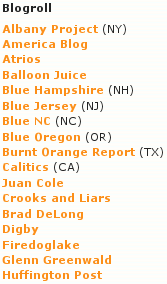
\includegraphics[width=\marginparwidth]{scrsh_dailykos_blogroll}
}

% While pointer pages still is in existance, it seems to use that 
% blog rolls is todays form of pointer pages.


\subsection{Item Annotation}
% tagging
% articles with tagging in context of social navigation
% lot of more discussion of tagging and mostly related to organizing
% principles and folksonomy

\subsection{Hyperlink Trails}
% bush, wexelblat99, new services, trailfire, new hoodwink.d greasemonkey
% service

\subsection{Collaborative Filtering}
% introduce earlier cited goldberg92 article and more recent work. recommender
% systems ties into this

\subsection{Visualization}
% activity, usage, edit/read wear

\subsection{Off the Web}
% security, mathematical models, etc

\section{Building on Top of the Web}
% greasemonkey, hoodwink.d, new hoodwink.d service
% browser extensions related, greasemonkey itself a extension, but
% thinking about specialized plugins for enabeling interaction on top of other
% web pages.
% mashups kind of related, maybe put inside web2.0 part or seperate part
% open apis is the fuel for mashups. possible without by screen sraping, but
% not as convenient and safe (upgrades on the pages we're scraping)
% facebook, open social. apps on top of social network sites. installed base
% of users and relationships already in place.

\section{Summary}

Based on our discussion of secondary background literature we've introduced
several terms:

\begin{description}
  \item[Web 2.0]
  \item[Social navigation]
  \item[Collaborative filtering]
  \item[Tagging]
  \item[More to come]
\end{description}
